% Seção: Modelagem
% Dono: Henrique · Orçamento: 2,5 página(s) · docs/fontes/plano-de-projeto.md §14.1
% Conteúdo: Modelo de dados, visões G_P, G_E, G_L e G_T, diagramas UML
% Fontes: docs/fontes/modelagem.md §3.4, docs/GUIA.md §8 (decisões D1 a D11 e piso de 1 s),
% src/transporte/modelo/. Figuras geradas de docs/diagramas/{classes-modelo,ge-exemplo}.puml.
% Condensada em 20/11 para o orçamento de 15 páginas.
\section{Modelagem}\label{sec:modelagem}

O GTFS~\cite{gtfs-reference} vira um \emph{modelo normalizado} e, dele, saem várias
\emph{visões} de grafo, cada uma escolhida pela pergunta que responde: nenhum grafo único serve
igualmente bem ao trajeto, às baldeações e à importância de uma parada.

\textbf{Modelo normalizado.} A \emph{parada} é um ponto de embarque, com identificador e
coordenadas. O \emph{padrão} é uma linha com uma sequência exata de paradas: variantes de
itinerário viram padrões distintos, porque as visões encadeiam as paradas numa ordem fixa. A
\emph{viagem} é uma passagem de um ônibus pelo padrão, guardada como a lista de horários em
cada parada, o que permite calcular o tempo entre duas paradas seguidas. Só entram as viagens de
um \emph{dia típico} (uma quarta-feira dentro da vigência do feed). Cada \texttt{stop\_id} é um
vértice próprio, mesmo quando o ponto físico tem uma parada por sentido; as duas ficam ligadas
por caminhada, o que preserva a travessia da rua.

\textbf{Visões.} Todas são grafos dirigidos e ponderados sobre a mesma estrutura própria, com
listas de adjacência e pesos em segundos (Tabela~\ref{tab:visoes}). Vértices e arestas podem ser
desativados sem reconstruir o grafo, o que a simulação de falhas usa. $G_P$ é a visão
estrutural, usada pelos algoritmos que percorrem a rede inteira; $G_L$ reduz as baldeações a uma
busca em largura entre padrões; $G_T$ é a extensão dependente do horário, FIFO, sobre a qual o
Dijkstra de chegada mais cedo continua correto.

\begin{table}[t]
\centering
\caption{Visões de grafo construídas a partir do modelo normalizado.}
\label{tab:visoes}
\footnotesize
\begin{tabularx}{\textwidth}{@{}l>{\raggedright\arraybackslash}p{2.6cm}%
  >{\raggedright\arraybackslash}X>{\raggedright\arraybackslash}p{3.0cm}@{}}
\toprule
Visão & Vértices & Arestas e pesos & Responde \\
\midrule
$G_P$ & Paradas & Viagem até a parada seguinte (tempo mediano); caminhada até
  $R$ metros (distância / velocidade) & Centralidades, eficiência, falhas \\
$G_E$ & Paradas e plataformas (parada, padrão) & Embarque (espera), viagem, desembarque
  (0) e caminhada & Trajeto mais rápido, espera \\
$G_L$ & Padrões & Dois padrões que compartilham parada ou têm paradas a distância de
  caminhada; sem peso & Mínimo de baldeações \\
$G_T$ & Paradas & Cada aresta guarda a lista de partidas; o custo depende do instante de
  chegada & Quadro de horários \\
\bottomrule
\end{tabularx}
\end{table}

\textbf{Por que $G_E$ existe.} Em $G_P$, continuar no mesmo ônibus e trocar de ônibus numa
parada custam o mesmo, porque a aresta não sabe em que linha o passageiro está. $G_E$ separa as
linhas em vértices de \emph{plataforma}, um por par (parada, padrão)
(Figura~\ref{fig:ge-exemplo}). Para trocar de linha, o passageiro desembarca (peso 0), volta ao
vértice da parada e paga uma nova aresta de embarque, com a espera $H/2$ da próxima linha
(Seção~\ref{sec:fund}). Assim um único Dijkstra soma caminhada, espera, viagem e baldeações, sem
penalidade arbitrária, e o número de baldeações é o de embarques menos um. Como o intervalo muda
ao longo do dia, $G_E$ é construído por faixa horária: pico da manhã (6h a 9h), entrepico (9h a
16h), pico da tarde (16h a 19h) e noite (19h a 24h). Um padrão sem partida na faixa não recebe
aresta de embarque nela.

\begin{figure}[t]
\centering
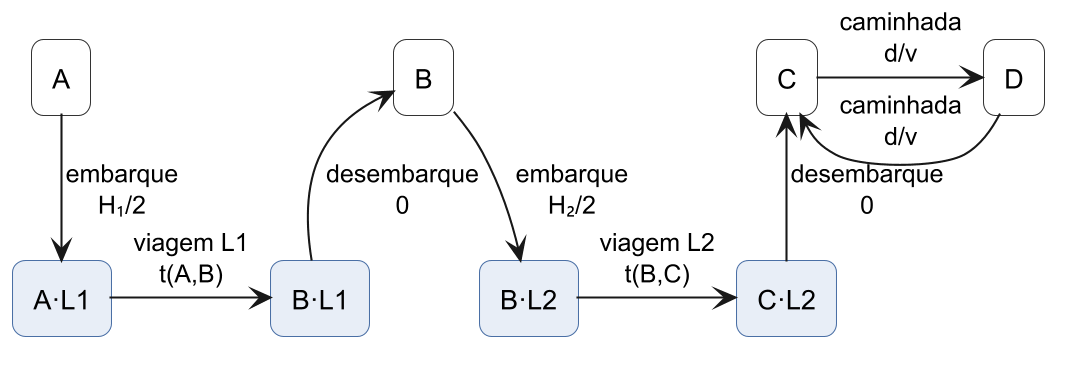
\includegraphics[width=0.46\textwidth]{ge-exemplo}
\caption{Exemplo de $G_E$: de A a C pela linha L1 e depois pela L2, com baldeação em B
(dois embarques); C e D estão a distância de caminhada. Em cima, as paradas; embaixo, em
azul, as plataformas.}
\label{fig:ge-exemplo}
\end{figure}

\textbf{Regras de construção.} O tempo entre duas paradas seguidas é a mediana das diferenças
de horário entre as viagens do dia, robusta a erros de cadastro; diferenças negativas ficam
fora. Em $G_P$, um trecho percorrido por dois padrões vira uma aresta única. A caminhada liga
paradas a até $R = 300$\,m em linha reta (haversine), a 1,2\,m/s. Arestas de viagem e de
caminhada têm piso de 1\,s: o GTFS arredonda horários, mas 0\,s entre paradas distintas é
artefato e quebraria a contagem de caminhos mínimos de Brandes. Uma grade espacial com células
do tamanho do raio reduz a busca dos pares de caminhada de $O(V^2)$ para $O(V + K)$ esperado,
com $K$ pares dentro do raio; construir $G_P$ custa $O(V + K + N \log N)$ e $G_E$,
$O(V + K + L + N \log N)$, com $N$ horários e $L$ plataformas.

No serviço de 04/11/2026, $G_P$ tem 9.659 vértices e 122.732 arestas (110.178 de caminhada) e
$G_E$ do pico da manhã, 46.100 vértices e 208.956 arestas; cada visão é construída em menos de
0,4\,s (Intel Core i5-13600KF, cinco execuções). O piso de 1\,s atinge 39 das 12.554 arestas de
viagem de $G_P$. Limitação: 387 dos 698 padrões repetem alguma parada, caso em que a
plataforma única por (parada, padrão) deixa seguir do fim para o início do padrão (as demais
estão na Seção~\ref{sec:conclusao}).

\textbf{Diagramas UML.} A Figura~\ref{fig:classes}a mostra as classes do modelo: o módulo
\texttt{construtores} lê a \texttt{Rede} e os \texttt{Parametros} e cria as visões, que herdam
de \texttt{Visao} e guardam um \texttt{Grafo} do núcleo e os mapas entre identificadores do
GTFS e vértices; a mesma figura traz o núcleo e os componentes, e a
Figura~\ref{fig:diagramas}, os diagramas de sequência e de atividade.

\begin{figure}[t]
\centering
\begin{minipage}[b]{0.39\linewidth}\centering
  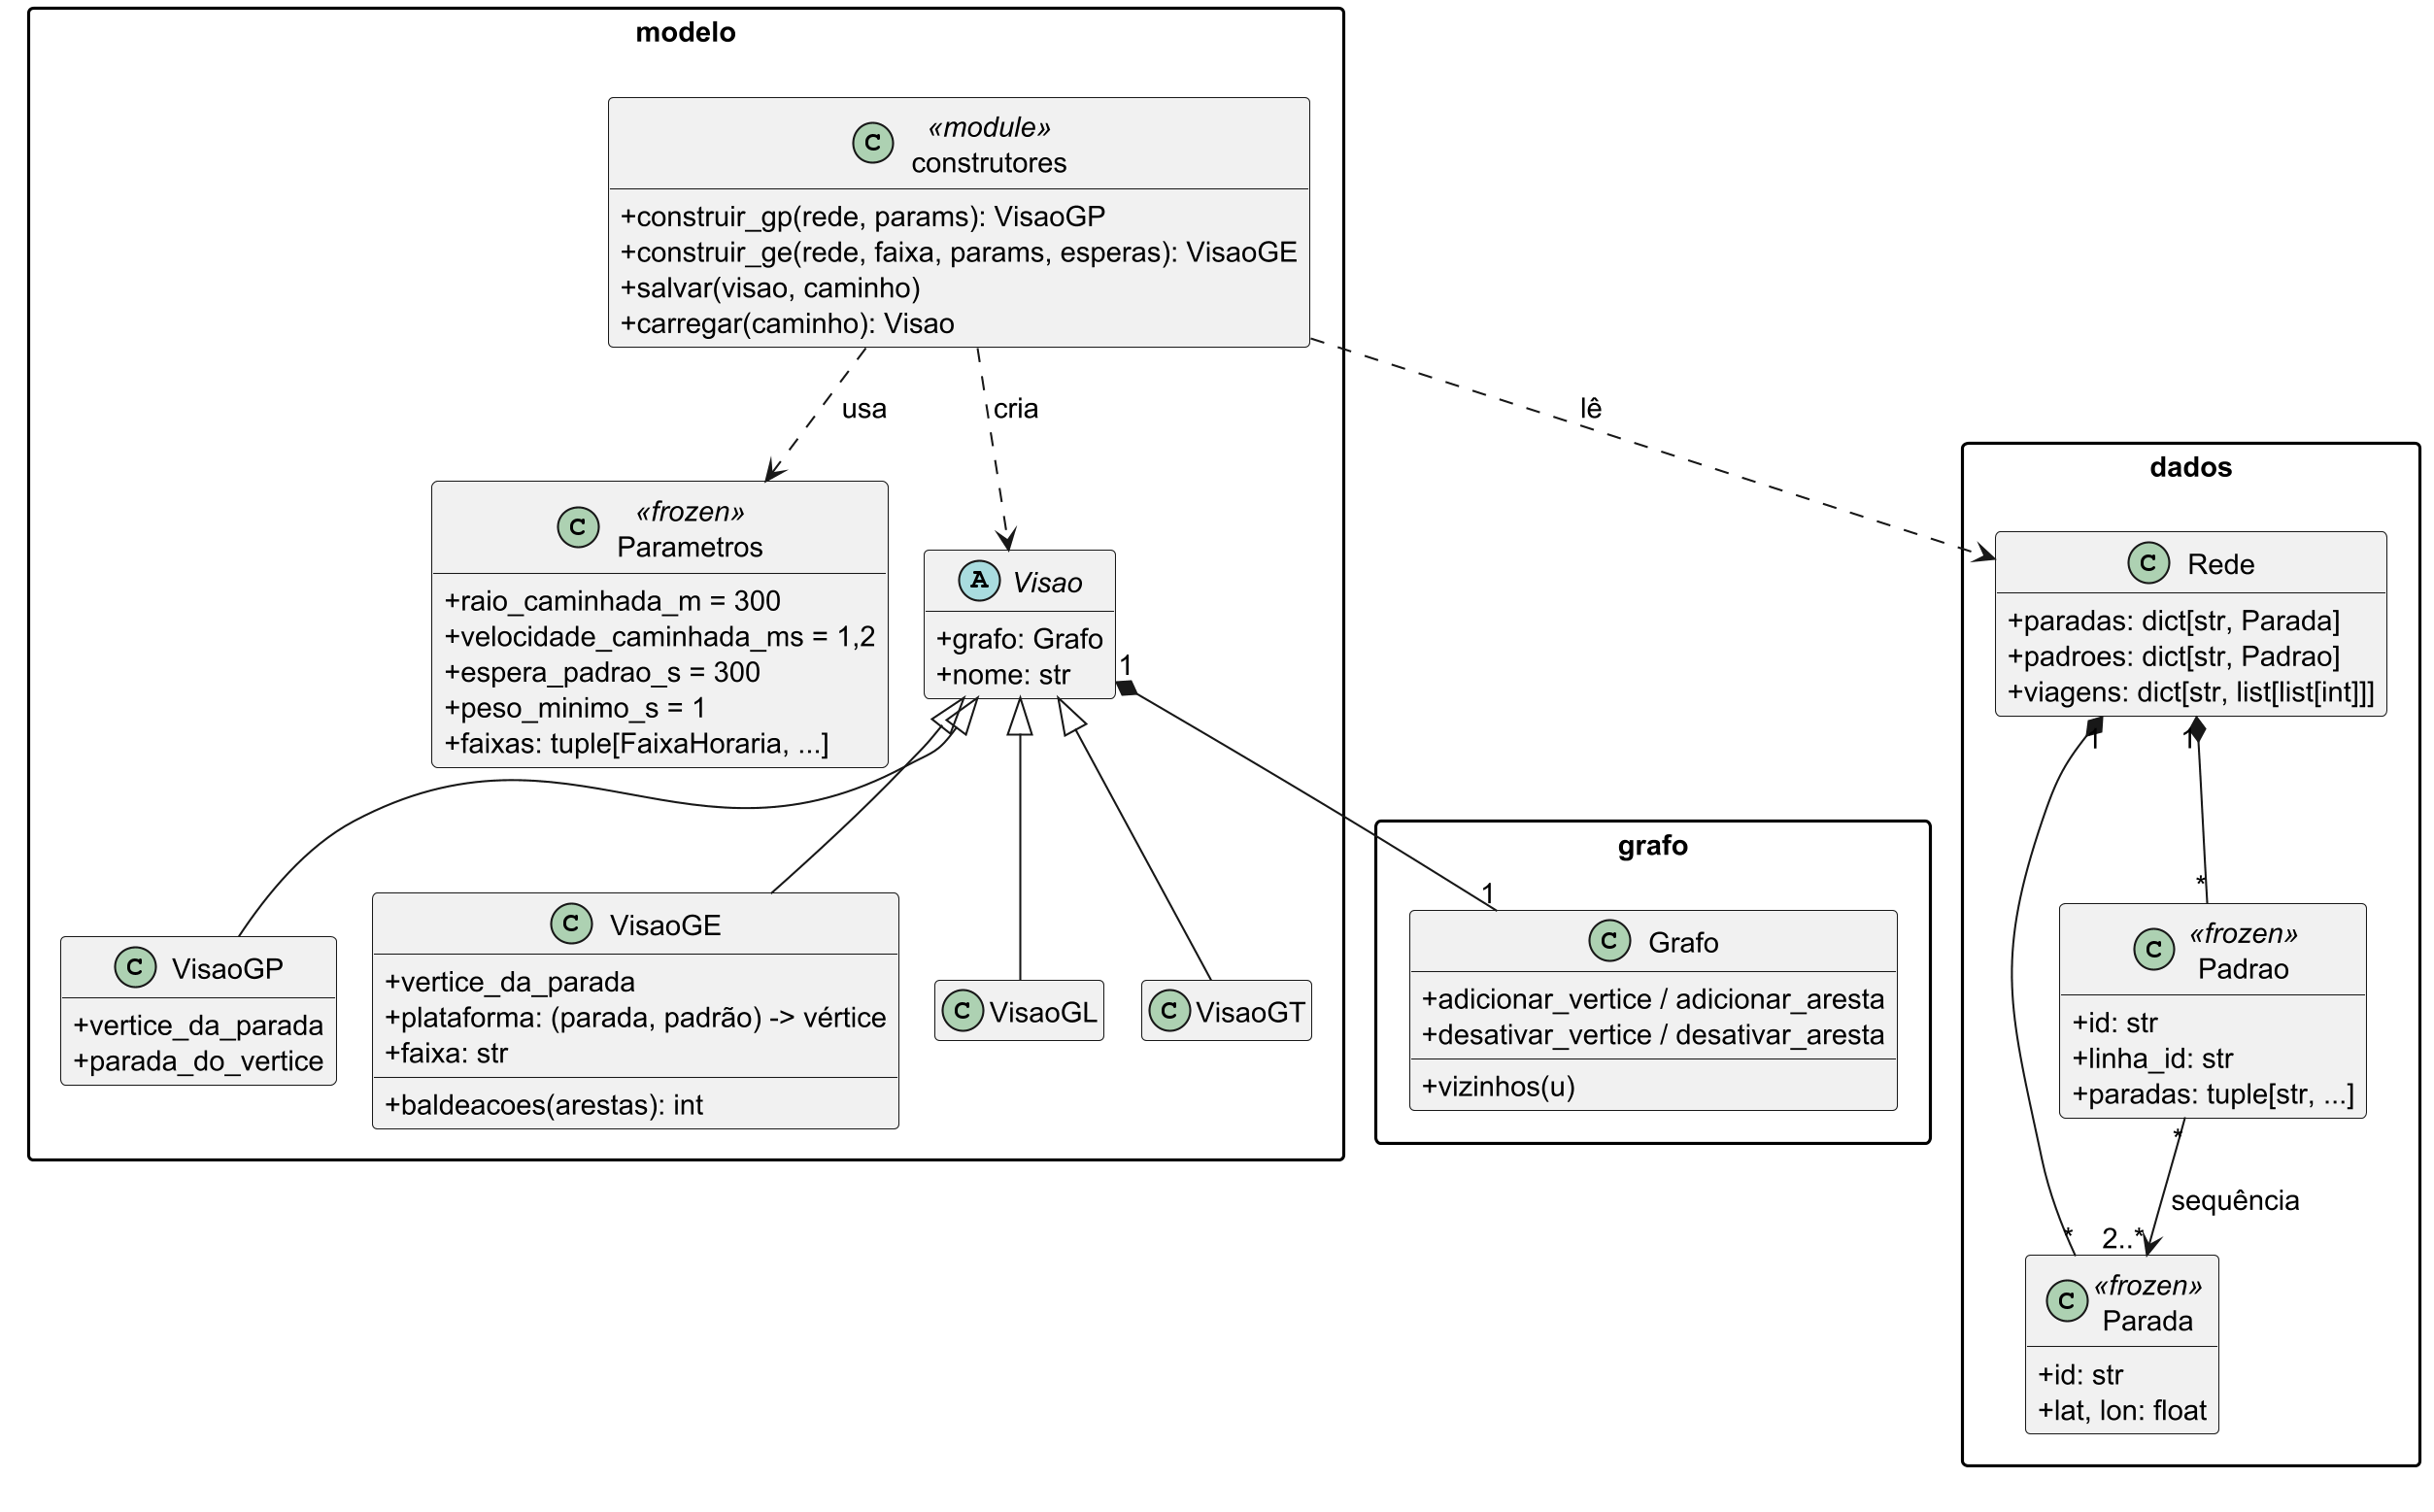
\includegraphics[width=\linewidth]{classes-modelo}\\{\scriptsize (a) Modelo, parâmetros e visões}
\end{minipage}\hfill
\begin{minipage}[b]{0.35\linewidth}\centering
  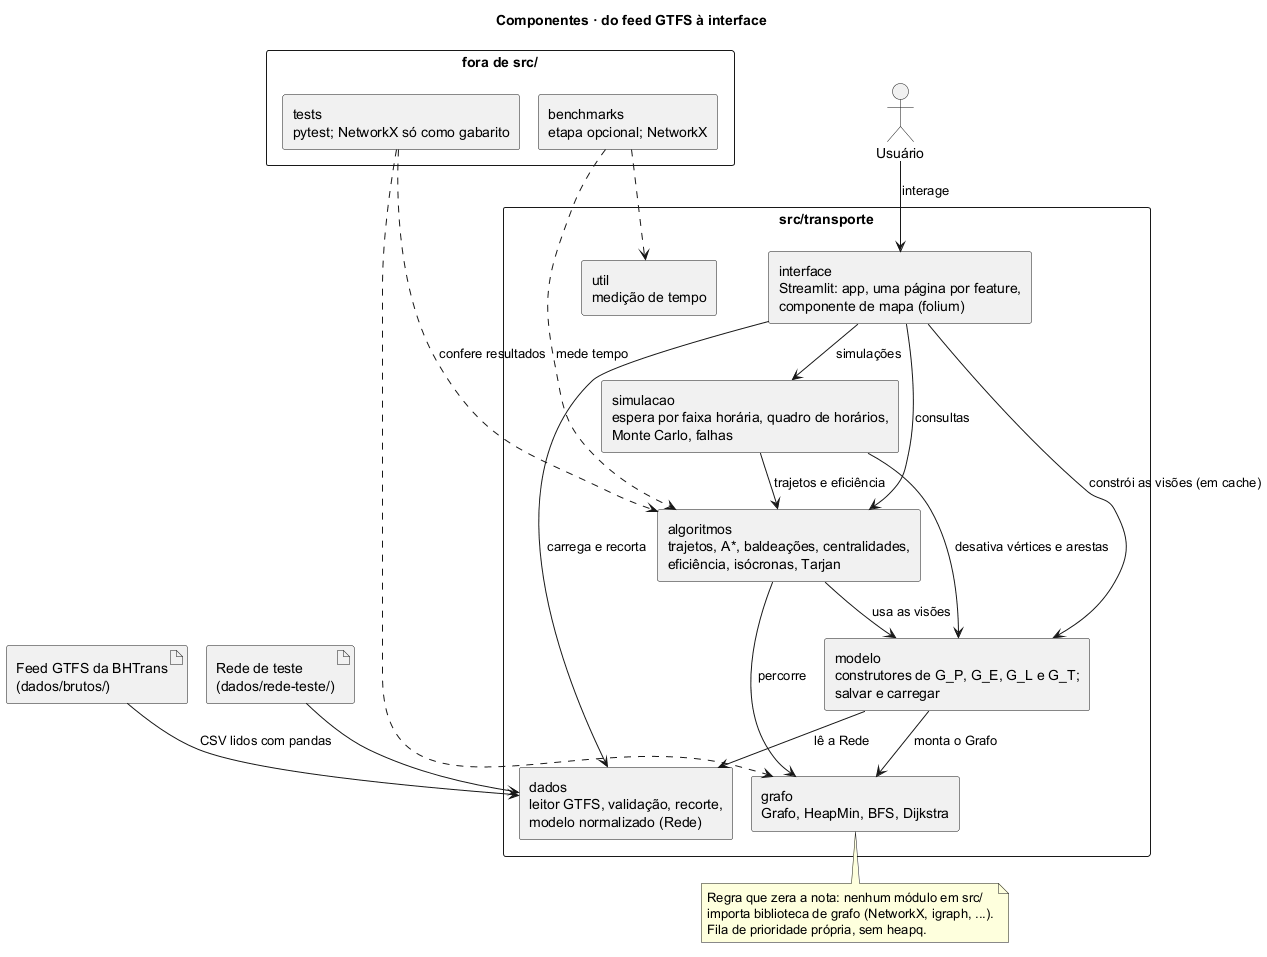
\includegraphics[width=\linewidth]{componentes}\\{\scriptsize (b) Componentes}
\end{minipage}\\[6pt]
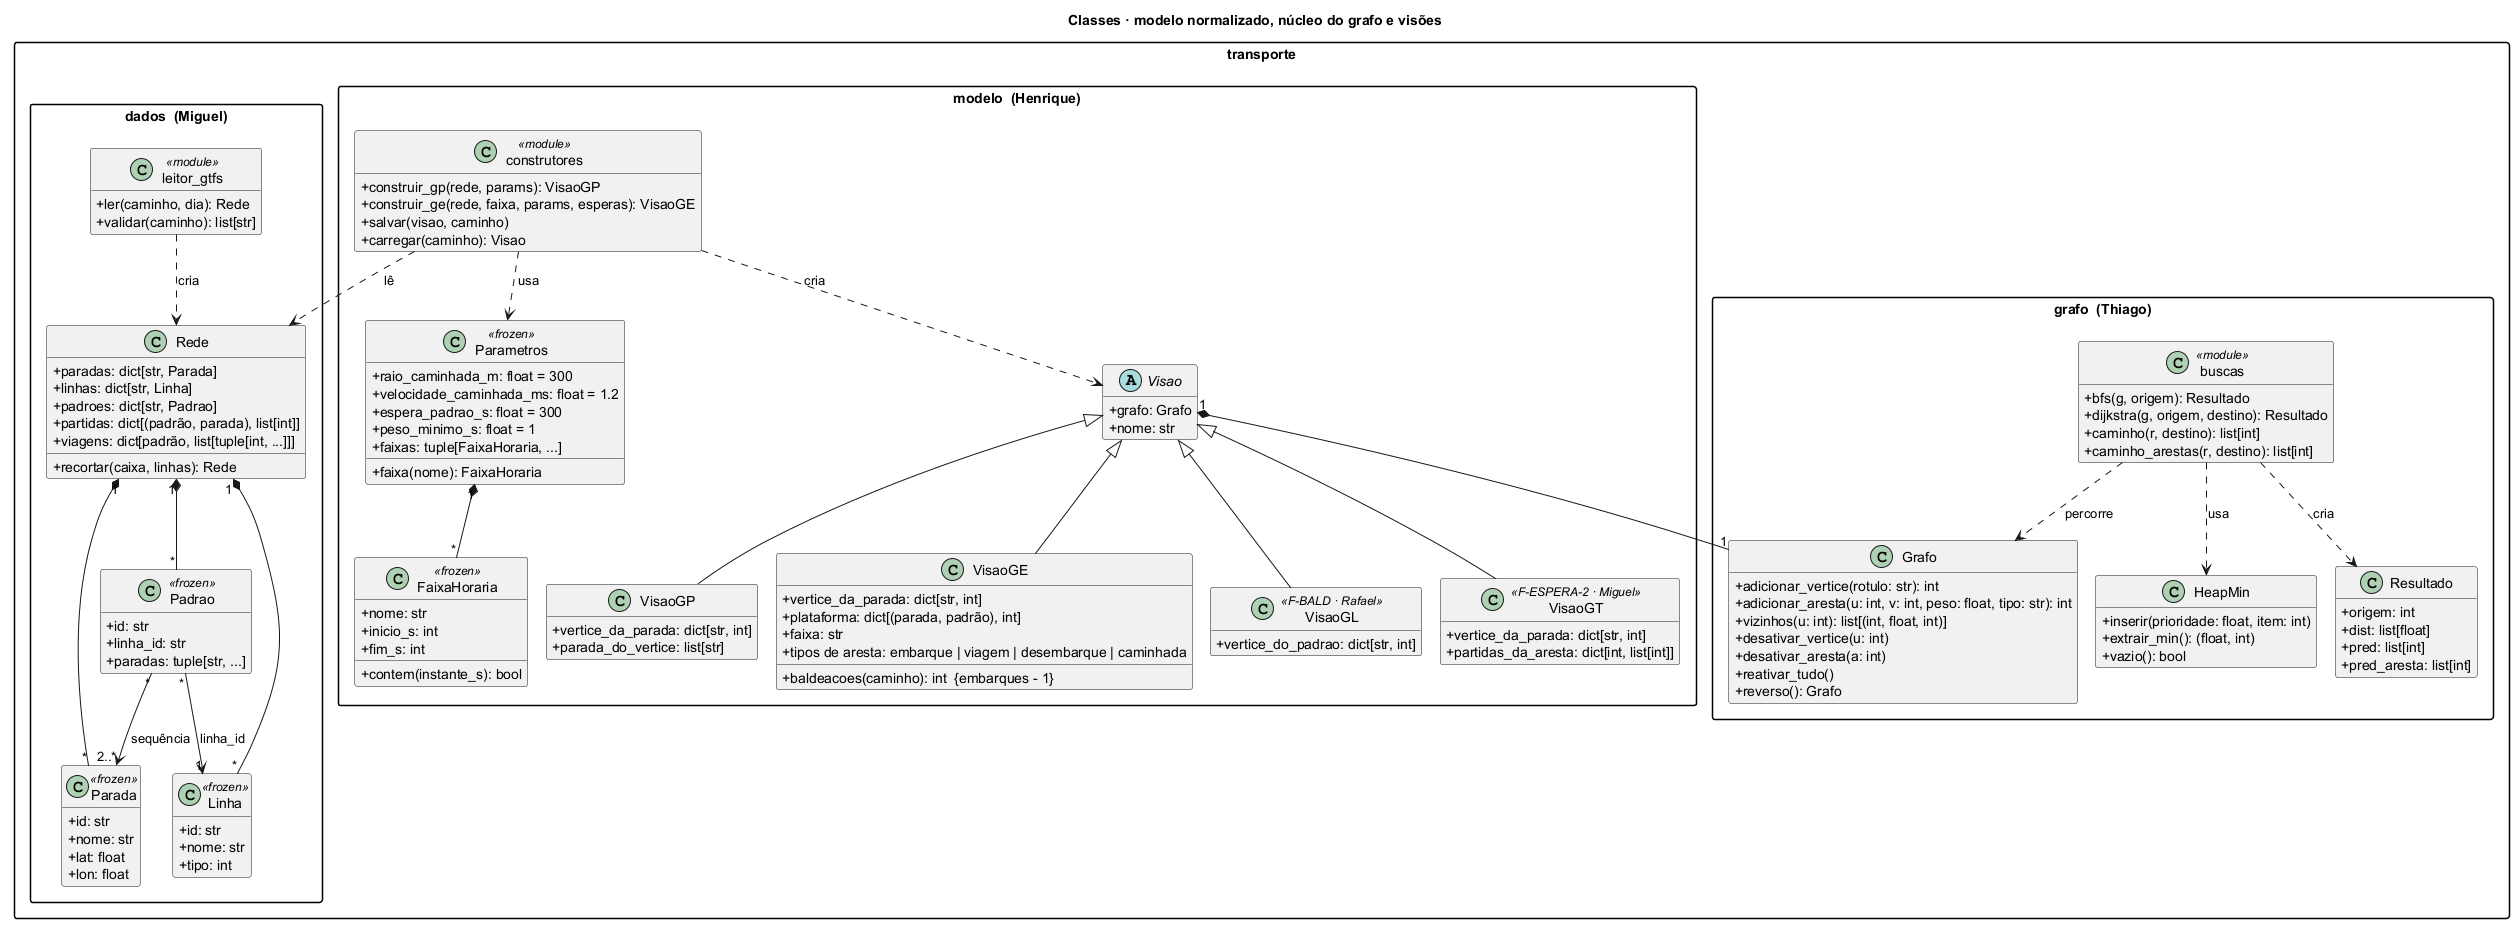
\includegraphics[width=0.74\linewidth]{classes}\\{\scriptsize (c) Classes do núcleo e das visões}
\caption{Diagramas de classes e de componentes.}
\label{fig:classes}
\end{figure}

% Diagramas UML das funcionalidades (sequência e atividade), em página própria.
% Dono: Henrique (integração) · fontes em docs/diagramas/*.puml, cópias PNG em figuras/.
% Incluída em 22/11 para cumprir o enunciado ("demonstrar todos os artefatos produzidos,
% como modelagem, diagramas, resultados obtidos e telas produzidas"). Os painéis são
% pequenos por causa do limite de 15 páginas; as imagens têm resolução para ampliar no PDF.

% \painel{arquivo}{largura}{altura}{legenda}
\newcommand{\painel}[4]{%
  \begin{minipage}[b]{#2\linewidth}\centering
    \includegraphics[width=\linewidth,height=#3\textheight,keepaspectratio]{#1}\\[-1pt]
    {\scriptsize #4}
  \end{minipage}}

\begin{figure}[p]
\centering
\textbf{\small Sequência}\\[2pt]
\painel{sequencia-dados-resumo}{0.30}{0.13}{(a) P0-DADOS}\hfill
\painel{sequencia-p0-ui}{0.20}{0.13}{(b) P0-UI}\hfill
\painel{sequencia-dijkstra}{0.22}{0.13}{(c) P0-GRAFO: Dijkstra}\hfill
\painel{sequencia-trajeto}{0.25}{0.13}{(d) F-ROTA: consulta}\\[5pt]
\painel{sequencia-trajetos-pagina}{0.30}{0.17}{(e) F-ROTA: página (A*, Yen)}\hfill
\painel{sequencia-eficiencia}{0.22}{0.17}{(f) F-EFI}\hfill
\painel{sequencia-falhas}{0.42}{0.17}{(g) F-RES: falha e Tarjan}\\[8pt]
\textbf{\small Atividade}\\[2pt]
\painel{atividade-p0-dados}{0.10}{0.27}{(h) P0-DADOS}\hfill
\painel{atividade-construir-ge}{0.15}{0.27}{(i) P0-MODELO}\hfill
\painel{atividade-medir}{0.12}{0.27}{(j) P0-AVAL}\hfill
\painel{atividade-intermediacao}{0.13}{0.27}{(k) F-MET}\hfill
\painel{atividade-menos-baldeacoes}{0.18}{0.27}{(l) F-BALD}\hfill
\painel{atividade-comparar-baldeacoes}{0.25}{0.27}{(m) F-BALD-2}\\[5pt]
\painel{atividade-espera}{0.24}{0.14}{(n) F-ESPERA: $H/2$}\hfill
\painel{atividade-quadro-horarios}{0.12}{0.14}{(o) F-ESPERA-2}\hfill
\IfFileExists{figuras/atividade-sensibilidade.png}{%
\painel{atividade-sensibilidade}{0.18}{0.14}{(p) F-ESPERA-OPC}\hfill}{}%
\painel{atividade-extensoes-eficiencia}{0.26}{0.14}{(q) F-EFI-2 e F-EFI-OPC}
\caption{Diagramas de sequência (a a g) e de atividade (h a q) das funcionalidades; fontes
PlantUML em \texttt{docs/diagramas/}.}
\label{fig:diagramas}
\end{figure}

